\chapter{Metodologia}

\begin{esboco}
Sociologia histórica processual

Métodos mistos

Séries temporais e análise de processos

Dados e Fontes
\end{esboco}

\section{Estratégias de comparação histórica e seleção de casos}\label{estratuxe9gias-de-comparauxe7uxe3o-histuxf3rica-e-seleuxe7uxe3o-de-casos}

A estratégia comparativa a ser empregada na investigação utilizará
diferentes lógicas de comparação \citep{tilly_big_1984} adequadas ao
estudo qualitativo de poucos casos (\emph{small-N}), individualmente
estudados via rastreamento de processos (\aiflag{Bennett e Checkel,
2015}; \citeauthor{mahoney_process_2015}, \citeyear{mahoney_process_2015})
e com ênfase na triangulação de dados quantitativos e qualitativos.
Dentro das abordagens sociológicas, há distintas formas de se pensar o
exercício comparativo, especialmente quando consideradas configurações
de nível macro. É importante deixar claro que essas distinções são
analíticas e muitas vezes os trabalhos se encontram nas fronteiras
dessas categorias ou são constituídos de múltiplas dessas estratégias
(\aiflag{Skocpol, 1984b}; \citeauthor{tilly_big_1984}, \citeyear{tilly_big_1984}).

Duas tipologias são bastante utilizadas, uma em \citet{tilly_big_1984} e
outra em \citet{skocpol_uses_1980}, especialmente naqueles que enfatizam
o caráter histórico das comparações. De sua parte, Tilly destaca
``grandes comparações'' sem enfatizar uma discussão de causalidade
\citep{tilly_big_1984}. O autor propõe quatro tipos de comparação:
universalizantes, de busca de variação, abrangentes e
individualizantes. Nesta investigação elas serão utilizadas como
estratégias para diferentes questões de pesquisa e escalas analíticas
específicas, dividindo-se o ``caso brasileiro'' da desindustrialização
em subcasos de forma a responder às distintas problemáticas.

Em primeiro lugar, pretende-se realizar comparações universalizantes,
orientadas a compreender a similaridade fundamental entre casos
distintos \citep[p.~83]{tilly_big_1984}. Respondem as perguntas: o que
há de comum nos processos de desindustrialização brasileiro ocorridos
aproximadamente de 1961 a 1967, 1986 a 1998 e de 2004\footnote{Aqui vale
  pontuar que, devido a diversas problemáticas relacionadas ao uso do
  critério de participação da indústria no PIB \aiflag{(Torres e
  Cavalieri, 2015)}, somadas às mudanças regulares metodológicas do
  sistema de contas nacionais, há obstáculos na estimação do processo de
  desindustrialização brasileiro \aiflag{(Morceiro, 2021)}. Como será
  discutido posteriormente, a abordagem mais comum para identificar o
  fenômeno da desindustrialização nos estudos brasileiros tem sido a
  participação do setor de manufatura no PIB. Esse dado será usado
  inicialmente como estimativa da periodização, mas parte significativa
  da tese envolverá reelaborar essa periodização com uso de dados de
  participação de outros setores industriais, crescimento real dos
  setores e emprego industrial.} em diante (B, E e G, cf. figura 2
abaixo)? Os períodos precedentes, de ciclos de industrialização ou
estabilidade (A, C, D e F, cf. figura 2 abaixo), possuem similaridades
que explicam os desenvolvimentos futuros?

\begin{figure}[htbp]
\centering
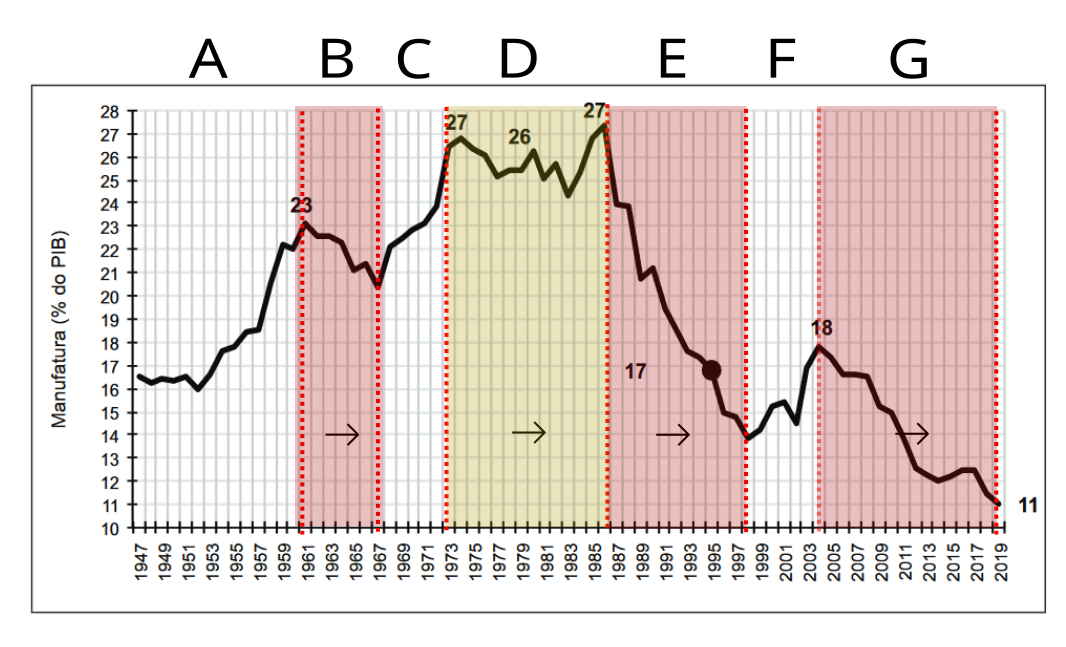
\includegraphics[width=\linewidth]{figures/cap03/periodizacao_industria_brasileira.png}
\caption{Periodização da trajetória industrial brasileira}
\label{fig:cap03-periodizacao}
\aiflag{Fonte: adaptado a partir de Morceiro (2021)}
\end{figure}

Em segundo lugar, serão são enfocadas as comparações em busca de
variação, a partir das quais tenta-se identificar um princípio de
variação, na intensidade ou tipo, de um mesmo fenômeno
\citep[p.~83]{tilly_big_1984}. Pergunta-se, então, qual a variação entre
subsetores industriais distintos (transformação, construção e
extrativo) diante das mesmas políticas públicas, contexto político e
cenário macroeconômico? Como a variação institucional entre estados
brasileiros líderes industriais (São Paulo e Rio de Janeiro) explica
mudanças na sua participação na indústria nacional nos mesmos períodos?

Por fim, a investigação mobilizará comparações abrangentes, que buscam
estabelecer as relações entre os casos como pertencente a um mesmo
sistema a partir de suas posições e características
\citep[p.~84]{tilly_big_1984}. Tais comparações aqui se refletem na
pergunta: como territórios produtivos passando por dinâmicas opostas
(ABC Paulista e Sul Fluminense) se relacionam enquanto parte de uma
mesma reorganização da indústria nacional?

Além das três estratégias mencionadas acima, há as comparações
individualizantes. Estas são comparações que visam identificar a
especificidade de um caso frente a um fenômeno
\citep[p.~83]{tilly_big_1984}. Apesar de não ser mobilizada aqui em
nenhum dos casos, na prática, o conjunto deste trabalho, baseado no
diálogo das três outras comparações, visa produzir em parte um olhar
detido sobre o caso brasileiro que pode ser lido como uma tentativa de
elaborar sua especificidade. Cada uma das lógicas acima se reflete
prioritariamente, portanto, em uma escala analítica prioritária
(nacional, estadual, sub-regional) ou na integração destas.

Paralelamente à definição de Tilly, \citet{skocpol_uses_1980}
elaboraram uma tipologia baseada em três estratégias comparativas. A
primeira diz respeito às estratégias de demonstração paralela, nas
quais dada teoria é identificada e tenta-se demonstrar sua
aplicabilidade a mais de um caso. É similar à lógica universalizante de
Tilly, apesar desta última enfatizar mais o caráter indutivo ao passo
que a demonstração paralela enfatiza o caráter dedutivo. A segunda
remete às estratégias de contraste de contextos, onde o objetivo é
identificar a especificidade de um caso, sendo assim similares à lógica
individualizante. A terceira são análises macro-causais, nas quais o se
busca identificar configurações causais que produzem dados resultados,
seja através da similaridade dos casos ou sua diferença. São similares
por vezes às lógicas de universalização, novamente, ou de busca de
variação, respectivamente.

Essa terceira estratégia, a macro-causal, portanto, se aproxima mais
claramente da estratégia desta investigação. Tal análise macro-causal é
bastante identificada com a sociologia histórica \aiflag{(Skocpol,
1984b)} e com a análise histórico comparativa
\citep{mahoney_comparative_2003-1}. Ela apresenta com frequência dois
desenhos de pesquisa comuns em estudos comparativos e que servem de
auxílio para a seleção de casos: a seleção de casos mais similares e a
seleção de casos mais diferentes \citep{skocpol_uses_1980}. Esse desenho
é baseado na obra de Stuart Mill, \emph{A System of Logic}, e reflete a
preocupação de um conjunto de autores com o elemento da causalidade, às
vezes denominado uma configuração causal. Sua proposição é que casos
para comparação deveriam ser selecionados quando tivessem resultados --
a variável dependente -- similares e compartilhassem apenas uma
característica -- a variável independente -- essencial. Ou,
alternativamente, quando tivessem resultados distintos, mas
compartilhassem de todas menos uma característica essencial. A
identificação dessas características chave permitiria ao pesquisador
elaborar a análise das causas necessárias e suficientes para o fenômeno
investigado.

Apesar da ampla defesa desse critério de seleção nos estudos
histórico-comparativos, é raro que estudos de fato consigam atingir
esses critérios estritos \aiflag{(Anckar, 2008)}. A seleção de casos
``mais similares'' ou ``mais diferentes'' é uma flexibilização dessa
regra de forma a permitir a análise \aiflag{(Perissinotto, 2023a)}. De
toda forma, continua improvável que os casos realmente sejam os mais
similares ou mais distintos possíveis \aiflag{(Perissinotto, 2023b)}.
Adicionalmente, o método apresenta limitações no que concerne fenômenos
com configurações multi causais -- isto é, em que diversas causas se
combinam para um mesmo resultado. Como resposta a necessidade de
comparação baseada na combinação de várias causas (i.e. variáveis
independentes), alguns autores propuseram o método QCA
(\citeauthor{ragin_comparative_2014}, \citeyear{ragin_comparative_2014};
\aiflag{Rihoux e Ragin, 2009}), mas este exige ou a ampliação do número
de casos (o que nem sempre é possível) ou o foco em menos variáveis (o
que nem é sempre desejável).

As técnicas inspiradas em Mill também são desafiadas por fenômenos que
podem possuir causas distintas com o mesmo resultado \aiflag{(Bennett e
Checkel, 2015, p. 201)} e quando há forte interação de variáveis
\citep{mahoney_strategies_2003}. Há ainda a questão de que o recorte
temporal pode alterar a definição da variável resultante ou o fato das
variáveis causais não terem presença homogênea no tempo. Por exemplo, em
contraste com países da Europa Ocidental e EUA, até meados dos anos 1980
o Brasil poderia ser entendido como um caso negativo de
desindustrialização. Posteriormente, podemos classificá-lo como um caso
positivo. Cabe então integrá-lo como um caso caracterizado por variáveis
muito distintas e resultado semelhante -- desindustrialização --,
assumindo recortes temporais distintos para cada país? Ou tratá-lo como
um caso de resultado distinto de outros países -- industrialização --,
mantendo o mesmo recorte temporal, incompleto no caso brasileiro, para
todos os casos?

Por fim, variáveis dependentes contínuas complexificam o problema de
definição de até que ponto as diferenças de intensidade em um fenômeno
consistem em resultados distintos. Todas as condições acima se aplicam
fortemente ao estudo da desindustrialização. A tabela 3 abaixo resume
alguns dos problemas lógicos do uso de similaridades e diferenças sem
análise de processos.

Como será discutido a frente, técnicas de rastreamento de processo são
bons recursos para compensar essas dificuldades sem sair do escopo de
pesquisas de amostragens pequenas. São particularmente adequadas para
análises históricas dada sua capacidade de reconstituir sequências
temporais, que são as unidades de análise e comparação. Tais técnicas
ajudam na medida em que permitem indutivamente identificar possíveis
variáveis omissas do caso ou verificar dedutivamente a causalidade de
uma variável para o resultado, sem necessariamente identificá-la como a
única variável distinta ou similar entre casos (\aiflag{Bennett e
Checkel, 2015}; \citeauthor{george_case_2005}, \citeyear{george_case_2005};
\citeauthor{mahoney_process_2015}, \citeyear{mahoney_process_2015}). É
baseado nessa premissa de que se fez a seleção de casos a partir da
variável dependente -- o processo de desindustrialização --, com fins de
ressaltar aspectos e dinâmicas mais importantes do fenômeno a ser
analisado. Isso não implica descarte da tentativa de uso, dentro do
possível, de maior similaridade ou maior diferença, mas sim sua
flexibilização necessária.

\begin{table}[htbp]
\centering
\caption{Problemas lógicos na seleção de casos mais similares e distintos}
\label{tab:cap03-problemas-logicos}
\csvautotabular{tables/cap03/problemas-logicos-selecao-casos.csv}
\end{table}

Nota: entre parênteses estão elementos causais.

Fonte: autoria própria

Também é importante notar que a seleção de casos (ou construção desses)
seguem estratégias distintas. Para as primeiras comparações, são
considerados recortes temporais de uma mesma sequência, o que implica
observação da influência de um caso no outro sempre numa mesma direção,
do passado ao presente. Para as comparações entre estados, as duas
sequências temporais são comparadas como independentes e paralelas
entre si. Para o caso das sub-regiões se inverte a lógica e a ênfase é
no aspecto relacional dos dois casos. A tabela 4 abaixo resume os casos
e suas percebidas similaridades e diferenças.

\begin{table}[htbp]
\centering
\caption{Casos analíticos e estratégia de seleção}
\label{tab:cap03-casos-estrategia}
\csvautotabular{tables/cap03/casos-analiticos-estrategia-selecao.csv}
\end{table}

Fonte: autoria própria

\section{Rastreamento de Processos e a comparação de sequências}\label{rastreamento-de-processos-e-a-comparauxe7uxe3o-de-sequuxeancias}

O uso de rastreamento de processos no âmbito sociologia histórica torna
central a discussão a respeito de análises de sequências ou análises
narrativas (\citep{abbott_sequences_1983}; \aiflag{Abbott, 1984, 1990};
\citeauthor{abell_narrative_2004}, \citeyear{abell_narrative_2004};
\citeauthor{clemens_toward_2007}, \citeyear{clemens_toward_2007};
\citeauthor{mahoneyfalleti2015}, \citeyear{mahoneyfalleti2015}). Esta é
fundamentalmente um diálogo entre ciências sociais e história buscando
combinar as lógicas de explicação centradas na temporalidade e no
contexto, típicas da história, com esforços de generalização ou
testagem teórica típicos das ciências sociais \citep{abbott_sequences_1983}.

\citet{abell_narrative_2004} chega a argumentar que o uso de explicações
narrativas constitui uma lógica distinta da explicação baseada em
variáveis, indicando uma relação entre dois estados do mundo distintos
conectados por arcos narrativos, a conexão causal entre esses dois
estados \citep[p.~1]{abell_narrative_2004}. De fato, a transição da
realização de análises comparativas baseadas em configurações
particulares de variáveis para aquelas preocupadas com processos
históricos sinaliza uma transição nas ciências sociais para uma
sociologia mais ``historicizada'' \citep{clemens_toward_2007} que
dialoga com questões importantes para vertentes institucionalistas,
estas preocupadas não apenas com efeitos de instituições congeladas no
tempo (causa X para um resultado Y), mas sim com mecanismos de auto
reprodução e de transformação institucional no tempo \aiflag{(Pierson,
2004)}, especialmente em seu diálogo com relações de poder
\aiflag{(Thelen, 2010)}.

Enfatiza-se, entretanto, que isso não impede o uso destas narrativas na
produção de generalização teórica ou comparação. O importante aqui é a
capacidade de produzir a generalização de ocorrências específicas de
uma sequência em eventos mais gerais. Assim, a análise da sequência de
eventos produz categorias comparáveis a outras sequências de eventos
\citep{mahoneyfalleti2015}. Variáveis reaparecem na linguagem enquanto
codificações desses eventos ou fatores externos que justamente influem
sobre os arcos narrativos, mas com durações distintas, naturezas
flexíveis e um leque, mesmo que institucionalmente constrangido, de
possíveis respostas dos atores. \citet{kreuzer_grammar_2023} enfatiza
esse diálogo ao propor a consideração tanto de tempos históricos -- as
sequências de eventos ordenados -- como do tempo físico -- a duração,
intensidade e ritmo dos processos -- em dois elementos a serem
combinados nas estratégias de análise histórico-comparativa.

A identificação desses eventos aqui irá constituir o centro da
estratégia analítica capaz de tornar transformações institucionais
distintas em categorias comparáveis analiticamente. Isso significa
empregar uma estratégia comparativa centrada no contexto
\citep{locke_apples_1995}, no qual a variável comparada em dados arcos
narrativos é determinada por sua significação. Por exemplo, diferentes
crises econômicas (inflacionária, de excesso de produção, interrupção
da produção) podem constituir um mesmo tipo de evento em distintos
arcos narrativos. É dessa forma que se poderá analisar se ``crises
econômicas'' são elemento explicativo do processo de
desindustrialização. Mas a questão, para além da presença desse evento,
é a relação entre sua duração, ordenamento temporal e as respostas dos
atores a ele. Assim, crises econômicas produzem desindustrialização,
hipoteticamente, na medida em que ocorrem em meio a determinados
contextos ou por determinado tempo de forma a produzir certas reações
dos atores, mas podem não fazê-lo quando essas reações forem distintas
ou os contextos não propícios a tal resultado.

Dada então essa importância da noção de processo para o entendimento
apropriado de cada caso, não é surpresa então que técnicas de
rastreamento de processo tenham se consolidado como método \emph{de
facto} de análises intra caso, componentes necessários para a posterior
análise entre casos \citep{mahoney_comparative-historical_2004}. O
rastreamento de processos visa a identificação das conexões causais
entre partes de um processo que formam o resultado final (\aiflag{Bennett
e Checkel, 2015}; \citeauthor{george_case_2005}, \citeyear{george_case_2005};
\citeauthor{mahoney_strategies_2003}, \citeyear{mahoney_strategies_2003}).
Seja em caráter dedutivo ou indutivo, este enfatiza o trabalho lógico de
reconstrução das etapas que levaram a um certo resultado, a própria
sequência temporal, portanto. Assim, diferente de métodos estatísticos,
na análise de processos toda a sequência causal deve estar demonstrada,
não bastando a presença da variável em uma dada quantidade de casos
(\aiflag{Bennett e Checkel, 2015}; \citeauthor{george_case_2005},
\citeyear{george_case_2005}).

Para isso, cada etapa de lógica exige a demonstração e teste da
conexão, de forma a tornar as hipóteses de conexão entre eventos
ordenados no tempo mais fortes \citep{mahoney_process_2015}. Para tal,
dois métodos mais populares têm sido identificados
\citep{mahoney_process_2015}. Primeiro, a identificação da presença de
evidência que fortemente apoia a conclusão, chamado teste da arma com
fumaça (\emph{smoking gun test}). Este teste não derruba hipóteses se
falhar. Quanto mais forte a evidência, mais confiança se tem na
hipótese. Em segundo lugar, aparece o teste de salto (\emph{hoop test)},
mais comum e no qual a ausência de certa evidência-chave derruba uma
hipótese. A princípio, sobreviver a um teste de salto não
necessariamente reforça a hipótese, mas sobreviver a uma série de
testes de saltos ou testes significativamente difíceis pode conferir
confiança a esta. Uma forma complementar de análise é trabalhar com
análises contrafactuais \citep{mahoney_comparative-historical_2004}, nas
quais os cenários ``alternativos'' hipotéticos servem para demonstrar o
efeito de dada variável.

Para exemplificar uma possibilidade, a análise de séries interrompidas,
baseada na projeção de uma série temporal antes de dada intervenção,
tem sido uma forma de análise contrafactual relevante para análise de
políticas públicas \aiflag{(Shin, 2017)}. Se combinarmos tal análise
com a análise qualitativa, por exemplo, de uma análise da relação entre
perfil ideológico de governantes e sua preferência por determinada
política pública, pode-se rastrear causalmente um dado resultado
econômico ou social ao perfil ideológico do representante eleito.
Assim, fica claro que o rastreamento de processos pode combinar
criativamente dados qualitativos e quantitativos.

Em resumo, o uso sistemático do método de rastreamento de processos
como parte da estratégia histórico-comparativa permite deslocar a
questão apenas da seleção de casos apropriados para comparação e em
direção aos métodos e técnicas de investigação intra casos, por exemplo
aquelas necessárias à compreensão de causas necessárias e suficientes
\citep{mahoney_strategies_2003,mahoney_comparative-historical_2004}.
Nesse cenário, os métodos de Mill não são suficientes para explicar
interação de variáveis ou múltiplas causas, mas ainda são úteis para
eliminar potenciais causas suficientes ou necessárias
\citep{mahoney_comparative-historical_2004}. De todo modo, a análise
intra caso se faz necessária para adequadamente compensar as
limitações da abordagem comparativa (idem).

Para concluir a seção, é preciso esboçar a estratégia integrativa entre
as diferentes escalas analíticas. Apesar do desenho dos objetivos e
capítulos sugerir uma escala do geral para o específico, na prática a
análise precisará ser iterativa entre os níveis. O contraste entre a
escala analítica superior e a inferior serve de forma a exacerbar as
características particulares dos casos de escala analítica inferior que
os fazem destoar do esperado. Assim, achados em escala mais baixa que
contrapunham achados em escala analítica mais alta sugerem necessidade
de revisões da mesma. Dito de outra forma, fatores explicativos do
processo em nível superior são considerados válidos para explicar as
similaridades entre casos analíticos de nível inferior, que são
considerados ``testes''. A existência de discrepâncias entre esses casos
gera a necessidade de estudo daquele caso, gerando novas proposições
explicativas sobre este e revisões das explicações sobre o caso de
nível superior.

\begin{figure}[htbp]
\centering
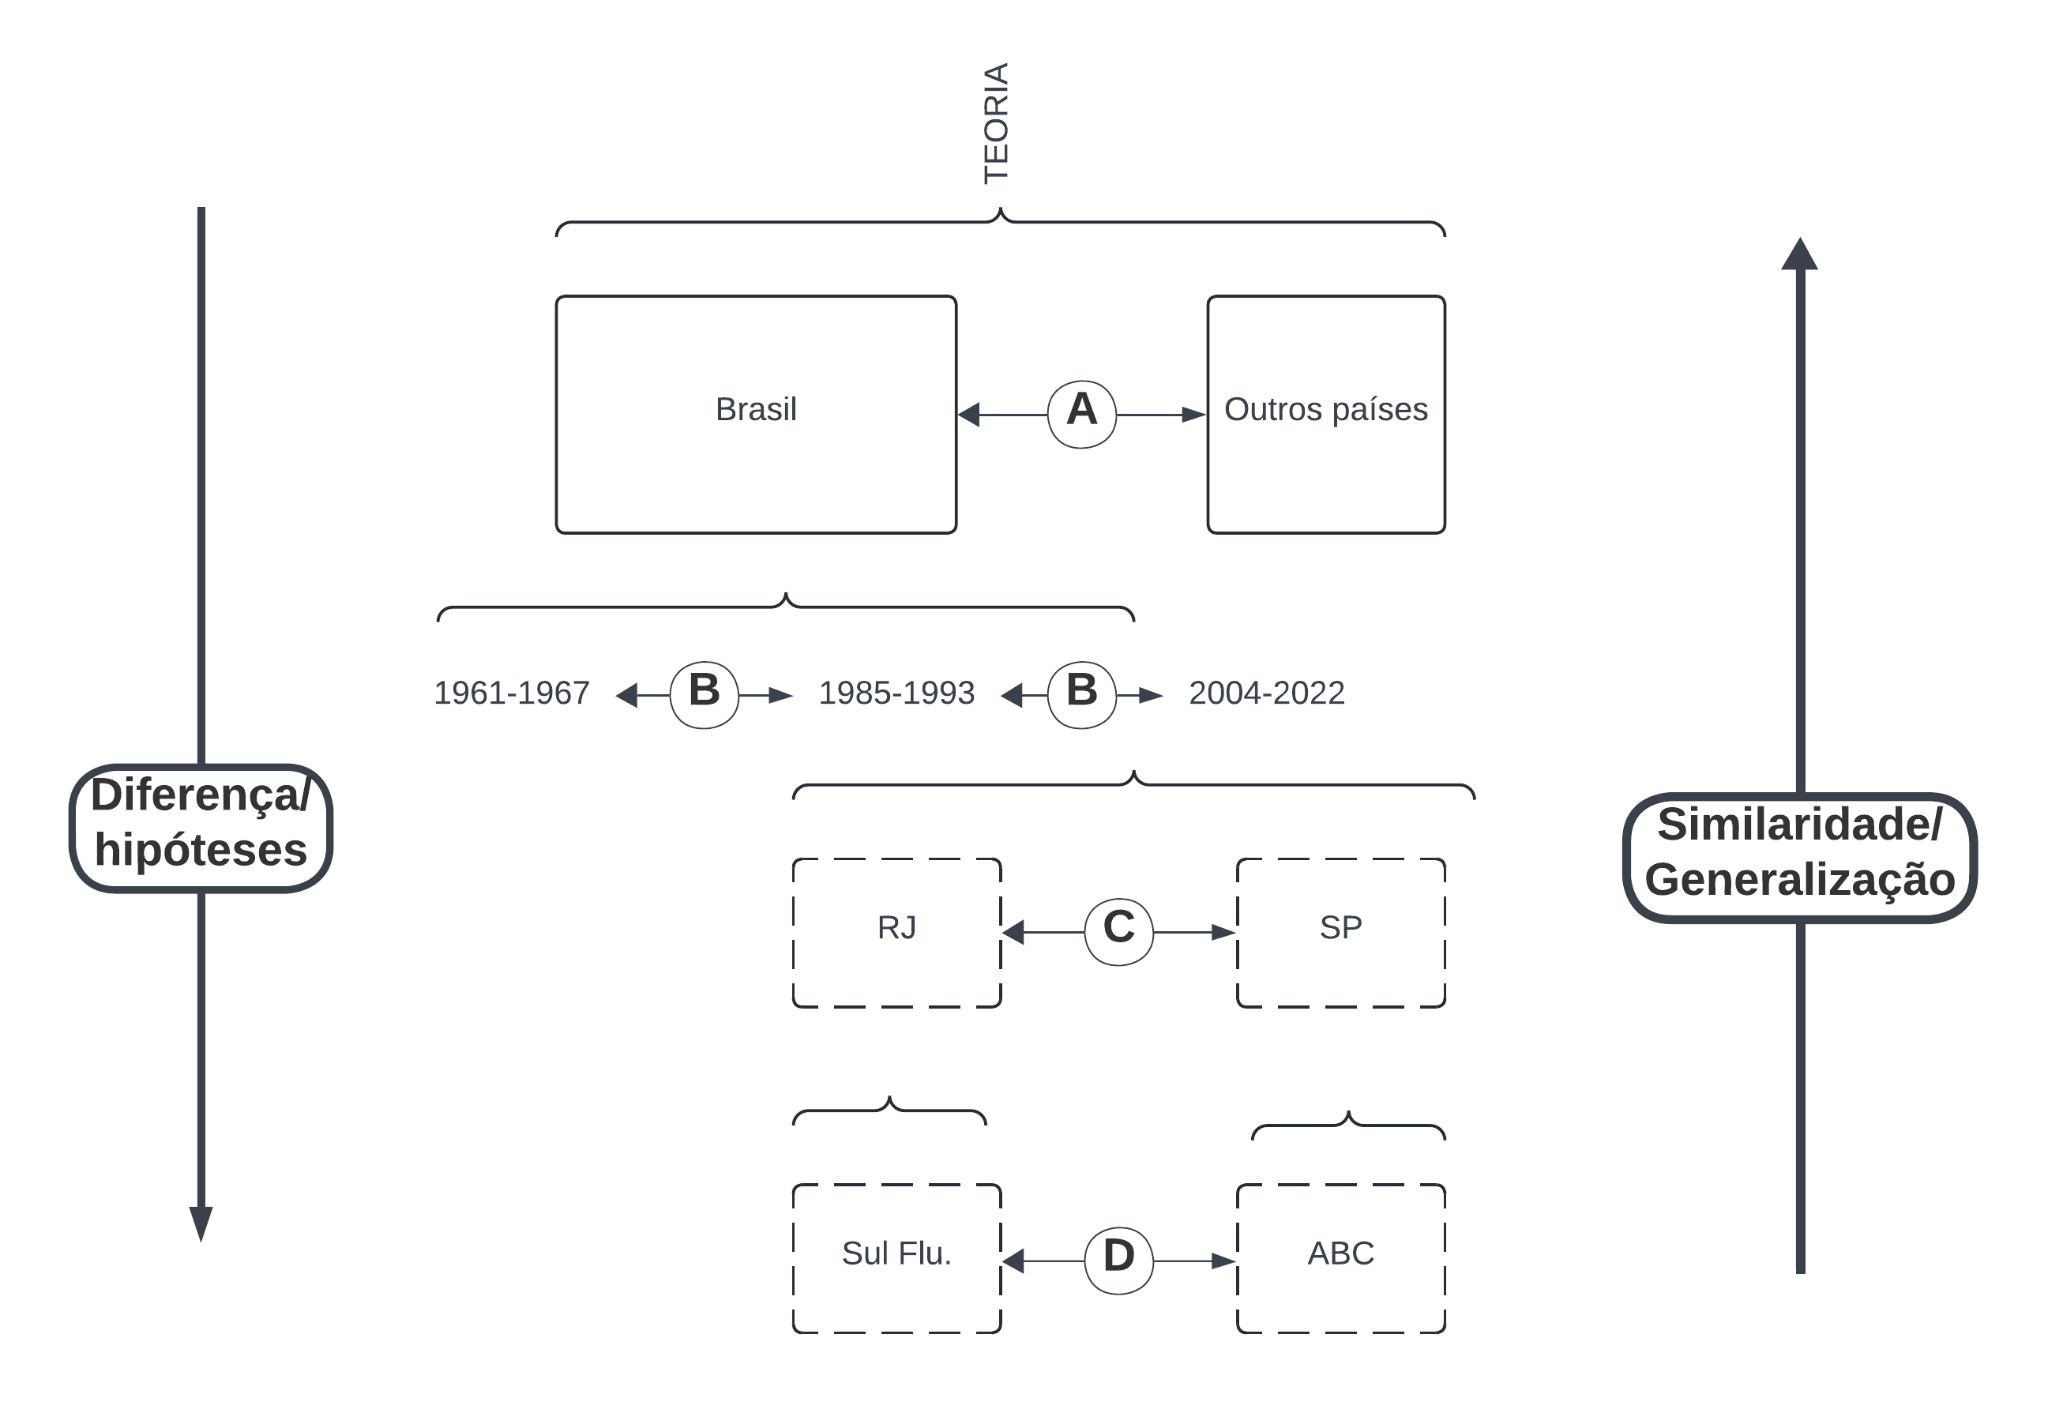
\includegraphics[width=\linewidth]{figures/cap03/estrategia_integrativa_niveis_analiticos.png}
\caption{Estratégia integrativa dos níveis analíticos e diferentes comparações (A, B, C e D)}
\label{fig:cap03-estrategia-integrativa}
\end{figure}

Fonte: autoria própria

\section{Recorte e indicadores}\label{recorte-e-indicadores}

A periodização proposta divide, a partir dos dados de participação da
indústria de transformação no PIB \aiflag{(Morceiro, 2021)}, o processo
de desindustrialização em diversas etapas (cf. figura 2, p.25). A
primeira sequência vai de 1961 até 1967. A segunda de 1986 até 1998,
sendo precedida por um período de estagnação entre 1973 e 1985. A
terceira vai de meados dos anos 2004 em diante. Propõe-se assim, como
ponto de partida o período prévio à primeira sequência, que marca o fim
de um período de crescimento econômico acelerado -- e forte
industrialização -- identificado com o pós segunda guerra mundial e os
governos Vargas e Juscelino Kubitschek. Dessa forma, o recorte temporal
total aproximado iria de 1951, com o segundo governo Vargas, até o fim
de 2023, imediatamente antes do lançamento do programa ``Nova Indústria
Brasil'' \citep{cndi_nova_2024}. Dado, entretanto, que a análise da
sequência temporal depende da identificação dos fatores chave para
esta, que será feita como parte da investigação, esse recorte temporal
não é imutável, servindo apenas de estimativa inicial.

Também já apresentados, os recortes geográficos são feitos na escala
nacional, estadual e sub-regional. Quando necessário, são trazidos de
forma pontual casos comparativos adicionais, por exemplo dados de
outros países ou estados brasileiros. Os recortes visam possibilitar
uma análise multiescalar do fenômeno. Como já dito, a alternância de
escalas é importante devido a presença de mecanismos institucionais
distintos nestas, por exemplo aqueles ligados à disputa fiscal entre
estados ou municípios.

\begin{table}[htbp]
\centering
\caption{Casos e recortes temporais}
\label{tab:cap03-casos-recortes}
\csvautotabular{tables/cap03/casos-recortes-temporais.csv}
\end{table}

Fonte: autoria própria

Quanto a indicadores do fenômeno, o principal indicador quantitativo
utilizado para estudos sobre desindustrialização no Brasil tem sido a
participação do setor industrial no PIB. Com frequência, os trabalhos
sobre o tema se concentram especificamente na participação da indústria
de transformação. Esse referencial, apesar de contribuições, tem
problemas e limitações \aiflag{(Torres e Cavalieri, 2015)},
especialmente no que concerne ao impacto da inflação nas suas
variações. Como apontado antes, é comum na literatura a ênfase sobre
volume de empregos de em adição a primeira métrica
\citep{tregenna_characterising_2009}.

Em complemento a esses dois indicadores, propõe-se utilizar
sistematicamente as taxas de crescimento real dos setores industriais,
calculadas a partir das Contas Regionais \aiflag{(IBGE, [s.d.])} e
Nacionais \aiflag{(IBGE, [s.d.])}, realizando comparação destes dados ao
crescimento real do PIB. O uso desse indicador é uma das contribuições
deste trabalho. Sua escolha se deve à sua capacidade de minimizar os
impactos da inflação na distorção e também capturar o ritmo pelo qual a
desindustrialização -- ou suas breves reversões -- tem ocorrido.

Alguns outros exemplos de indicadores estão também presentes na
literatura e podem ser mobilizados pontualmente. São eles o número de
estabelecimentos industriais \aiflag{(Sobral, 2016)}, os investimentos
produtivos \aiflag{(Curado e Cruz, 2008; Dávila-Fernández, 2015)}, os
resultados da balança comercial \citep{marconi_taxa_2012}, os dados
brutos da produção industrial \aiflag{(Sobral, 2017)} e os dados sobre
diversidade ou dispersão da atividade industrial \aiflag{(Morceiro e
Guilhoto, 2020)}. A tabela abaixo condensa algumas das vantagens e
desvantagens dos indicadores.

\begin{table}[htbp]
\centering
\caption{Indicadores de desindustrialização na literatura}
\label{tab:cap03-indicadores-literatura}
\csvautotabular{tables/cap03/indicadores-desindustrializacao-literatura.csv}
\end{table}

Fonte: autoria própria

\section{Variáveis, unidades de análise e atores}\label{variuxe1veis-unidades-de-anuxe1lise-e-atores}

As instituições analisadas, e suas transformações constituem as
principais variáveis independentes do modelo, com as quais o processo
de desindustrialização se relaciona. Elas precisam ser gerais o
suficiente para serem percebidas como condicionantes da ação de atores
coletivos em detrimento das variações e preferências individuais de
seus membros. Elas também não podem apenas emergir da agregação de
indivíduos, como parte de suas psicologias individuais. Uma forma de
operacionalizar o conjunto de instituições a serem analisadas é
trabalhar com a proposta de níveis institucionais de \aiflag{Fligstein e
Choo (2005)}, utilizada para a análise da governança corporativa.
Assim, os autores diferenciam estruturas muito amplas e dispersas na
sociedade, o sistema político, a economia e a cultura, das instituições
ao nível das normas (para eles as referentes à governança e legislação)
e de suas manifestações no nível das práticas. Aqui é esse nível
intermediário, da ``norma'' que guia a escolha de instituições, mesmo
que estas operem em diferentes escalas geográficas. Assim, são
removidas da discussão instituições muito próximas da dimensão da
prática, como o aperto de mão, e ao mesmo tempo os aspectos
institucionais muito amplos, como características institucionais do
capitalismo, por exemplo a ``ganância'' ou ``auto interesse'', como
propostas por Streeck \aiflag{(2011, 2012)}.

Abaixo se apresenta uma listagem esquemática dos conjuntos de
instituições preliminarmente consideradas mais relevantes, com sua
caracterização e escala (cf. tabela 7 abaixo). Aqui é feita uma
diferenciação entre instituições e atores, sabendo que essa distinção
não representa uma dicotomia real. Instituições transpassam atores,
sendo às vezes internas ou externas a estes \aiflag{(Santos, 2019)}. De
outra forma, como \citet{morgan_actors_2010} pontua, instituições e
atores são co-constitutivos. Esses fatores são relevantes pois são
frequentemente origem das transformações endógenas nessas instituições.
Isso implica inserir uma discussão sobre poder na análise institucional
\aiflag{(Thelen, 2010)}. Nesse sentido, não se trata apenas de atores
operando racionalmente, mesmo que tal racionalidade seja contextualmente
limitada, perante instituições externas, mas, como Scharpf
\aiflag{(2018, p. 39)} argumenta, de atores coletivos que apenas existem
e podem operar pois seus membros individuais coordenam suas ações
frente a um referencial institucional. Assim, instituições são externas
e internas aos atores. São ao mesmo tempo resultado de suas ações e
condição de sua existência.

\begin{table}[htbp]
\centering
\caption{Conjuntos preliminares de instituições relevantes}
\label{tab:cap03-conjuntos-instituicoes}
\csvautotabular{tables/cap03/conjuntos-instituicoes-relevantes.csv}
\end{table}

Fonte: autoria própria, instituições econômicas formuladas a partir de
Santos \aiflag{(2024)}.

Por sua vez, as fontes de mudanças exógenas foram classificadas como
``choques externos'' e na tabela 8 (página 28-29) também é apresentada
uma breve esquematização das variáveis consideradas como indicadores
desses choques\footnote{Alguns outros eventos ou choques que podem ser
  de antemão esquematizados: Boom econômico nacional; Boom econômico
  internacional; Crise econômica nacional; Crise cambial internacional;
  Boom de commodities.}, sendo seu impacto ou não nas instituições uma
questão empírica. Como mencionado, a proposta é generalizar ocorrências
específicas em categorias de eventos que sejam comparáveis entre
sequências temporais distintas \citep{mahoneyfalleti2015}. Por exemplo,
diversas crises econômicas internacionais podem ser classificadas no
tipo de evento ``crise econômica externa''.

Os eventos podem ser analisados considerando sua duração e sequência
\citep{mahoneyfalleti2015}. Assim, a título de exemplo, a longa duração
da crise inflacionária brasileira dos anos 1980 é relevante para
entender seus impactos. Da mesma forma, a precedência da crise das
\emph{commodities} em relação ao impeachment de Dilma Rousseff também é
fator relevante. Alguns desses eventos podem ser considerados
causalmente necessários ou suficientes a outros, enquanto algumas
sequências temporais podem meramente ser ordenadas, sem causalidade
necessária (\aiflag{Abbott, 1984}; \citeauthor{mahoneyfalleti2015},
\citeyear{mahoneyfalleti2015}). A consideração das sequências de
eventos, em algum grau generalizáveis, permite a constituição de uma
narrativa verossimilhante que pode ser utilizada como fator explicativo
\citep{abell_narrative_2004}. Por sua vez, o próprio caráter de
``processo'' implica um tipo específico de sequência na qual ``os
eventos ordenados pertencem a um dado tipo de atividade''
\citep[p.~214]{mahoneyfalleti2015}\footnote{Tradução própria}.

\begin{table}[htbp]
\centering
\caption{Categorias de eventos relativos a ``choques externos''}
\label{tab:cap03-choques-externos}
\csvautotabular{tables/cap03/categorias-choques-externos.csv}
\end{table}

Fonte: autoria própria

Nesse ponto, vale reforçar que, se instituições são as variáveis, a
unidade de análise são as sequências temporais. De fato,
\citet{mahoneyfalleti2015} argumentam que a unidade de análise básica
das comparações históricas são as sequências. Isso permite exercitar um
conjunto de observações e comparações mesmo internamente a um único
caso, na medida em que diversas sequências podem ocorrer em paralelo
\citep{mahoneyfalleti2015}. Assim, novamente em caráter ilustrativo, o
processo de desindustrialização poderia ser lido como duas sequências
paralelas, uma de transformações tecnológicas e outra relativa às
transformações nas relações de trabalho, que se reforçam mutuamente,
permitindo uma drástica redução da força de trabalho industrial. Essa
concepção ajuda a evitar narrativas excessivamente deterministas sobre
os processos.

Por fim, pode-se esquematizar provisoriamente os conjuntos de atores
considerados mais relevantes. Como discutido, instituições são
frequentemente transversais a atores e sua compreensão precisa ser
mútua de forma a compreender a racionalidade dos segundos
(\aiflag{Santos, 2019}; \aiflag{Scharpf, 2018}). De toda forma, o elenco
de atores capazes de influenciar significativamente as instituições (ou
ser diretamente influenciado por elas) depende da definição das mesmas
e da escala analítica considerada.

Entre os atores ligados ao Estado considerados relevantes estão, então,
o poder público na forma dos governos em níveis federal, estadual e
municipal, além do poder legislativo e outras organizações ligadas ao
Estado, como o Ministério Público. Optou-se por não tratar o Estado como
um ator único e sim um conjunto de atores/organizações. Enfatiza-se que,
em que pese a existência de políticas de Estado transversais a diversos
governos, no caso brasileiro a especificidade de cada governo é
relevante para entender sua relação com a questão do desenvolvimento
econômico e indústria. Assim, é dada ênfase à particularidade
ideológica e também ao interesse político e econômico dos poderes
executivo e legislativo, seus principais representantes e membros, em
diferentes níveis e momentos.

São também relevantes as empresas e suas estratégias corporativas
\aiflag{(Santos e Ramalho, 2015)}. Estas por vezes se articulam em
associações empresariais de forma a mais diretamente buscar influenciar
os rumos das políticas de seus respectivos setores. É importante
compreender aqui os contextos de racionalidade desses atores
econômicos, mais do que suas estratégias particulares. Assim, padrões
de estratégias corporativas -- como busca de flexibilização, realocação
produtiva, ciclos de investimento, etc -- são consideradas frente a
contextos políticos e econômicos.

Do ponto de vista da sociedade civil, movimentos sociais são
considerados importantes articuladores das demandas sociais. Assim,
acabam por exercer pressão tanto sobre o Estado como sobre as empresas e
suas estratégias. Entre os movimentos sociais considerados, é dada
primazia à análise do papel de sindicatos, devido a sua articulação mais
direta com as questões do emprego e do desenvolvimento econômico.

Por fim, atores ``externos'' de caráter transnacional são também
importantes na medida em que são balizadores de instituições fortemente
influentes. Exemplos disso são o Fundo Monetário Internacional (FMI), a
Organização Mundial do Comércio (OMC) e as agências de classificação de
risco. Esses atores se relacionam a instituições significativas na
escala nacional, a saber: a gestão da dívida externa e também a
política fiscal do governo por parte do FMI; as políticas de comércio
externo e subsídios a setores específicos, a qual se relaciona a OMC; a
classificação de risco do país por parte das agências classificadoras,
que determina regras para investimento externo no país e também
normatiza, do ponto de vista de investidores externos, a política
econômica e fiscal ``desejável''.

\section{Materiais e métodos}\label{materiais-e-muxe9todos}

A partir dos indicadores anteriormente mencionados, pode ser
estabelecida uma tabela de dados quantitativos a serem coletados e suas
respectivas fontes. Inicialmente se utilizarão os dados sempre
disponibilizados anualmente, mas caso necessário é possível agregar
dados de periodicidade mais curta.

\begin{table}[htbp]
\centering
\caption{Indicadores quantitativos e fontes}
\label{tab:cap03-indicadores-quantitativos}
\csvautotabular{tables/cap03/indicadores-quantitativos-fontes.csv}
\end{table}

Fonte: autoria própria

A estratégia de análise dos dados quantitativos será a análise de
séries temporais \aiflag{(Shin, 2017)}. Dentro desta será enfatizada a
análise gráfica de tendência a partir de médias móveis e, em alguns
casos, o uso de regressões lineares múltiplas para verificar o peso de
dada variável. Também será analisada a correlação entre conjuntos de
séries temporais.

Já o conjunto de dados qualitativos a serem coletados e analisados é
provisoriamente esquematizado, de forma não exaustiva, na tabela a
seguir. Apenas serão trabalhadas de forma sistemática as fontes
primárias relativas a alguns conjuntos de instituições. Para outras
instituições, atores coletivos e choques externos será utilizada de
pesquisa bibliográfica de forma a consolidar dados de fontes
secundárias. A estratégia de análise do material será a análise
documental \aiflag{(Bowen, 2009)}.

\begin{table}[htbp]
\centering
\caption{Fontes de dados qualitativos}
\label{tab:cap03-fontes-qualitativas}
\csvautotabular{tables/cap03/fontes-dados-qualitativos.csv}
\end{table}

Fonte: autoria própria
